\documentclass{aa}
\usepackage[varg]{txfonts}
\usepackage{siunitx}

\DeclareSIUnit\Rsol{R_\odot}
\DeclareSIUnit\AU{AU}

\begin{document}


\title{Assignment 1}

\subtitle{Introduction and visualization}

\author{David Hernandez\inst{1}
}

%\offprints{R. Plemmons, \email{plemmons@... plemmons@...}

\institute{Universit\"at Wien, Institut für Astrophysik, T\"urkenschanzstrasse
17, 1180 Wien, Austria
}

\date{Deadline: unknown / Submitted: \today}

\abstract{As a first introduction to numerical computation, three different
methods were implemented and tested. The first method is a numerical integrator
using simpsons rule. The numerical integration concludes the first part, whereas
the second part takes a closer look at two different approaches to function
solving. One implementaition was done by using the Newton iteration andthe 
second was realized with the bisection method. Since the latter are both
iterative, recursion was favoured over loops in order to achive a performance
boost. However, no benchmarking was done, so it might be possible, that a
solution involving loops could be just as fast if not faster.}

\keywords{keyword1 -- keyword2 -- keyword3 -- keyword4 
-- keyword5 -- keyword6}
\maketitle 

\section{Simpson integration}%
\label{sec:simpson_integration}

Numerical integration using Simpsons rule is done by dividing the interval \([a,
b]\) into individual subintervals. The number of these subintervals are
basically the integration steps. The accuracy of the result increases with a
growing number of steps. To get to the solution, we need to compute the
function value at three point in step, at the beginning, the middle and the end.
Therefore, if we have only one integration step, for the integral
\begin{equation}
    \int\limits_a^b f(x) dx 
\end{equation}
we compute \(f(a)\), \(f((b-a)/2)\) and \(f(b)\). This special case with only
one integration step is also known as Kepler integration.
\begin{equation}
    \int\limits_a^b f(x) dx \approx \frac{b - a}{6} \left(f(a) + 
    4~f\left(\frac{b + a}{2}\right) + f(b)\right)
\end{equation}
If we now want to adapt this for \(n\) integration steps we get the following:
\begin{equation}
    \label{equ:simpson}
    \begin{split}
        \int\limits_a^b f(x) dx \approx \frac{\Delta x}{6} 
        \bigg[f_0 + f_{2n} & + 4\Big(f_1 + f_3 + \dots + f_{2n-1}\Big) \\
        & + 2\Big(f_2 + f_4 + \dots + f_{2n-2}\Big)\bigg]
    \end{split}
\end{equation}
This scheme assumes that there are \(2*n + 1\) evaluation points for the
function that shall be integrated. Therefore, the first implementing this method
is to work out the number of evaluation points from the number of integration
steps. Next we have to determine the width \(\Delta x = (b - a)/2\) of the
individual steps. In the script the function values of all evaluation points are
stored into a \verb+numpy.array\verb+ object. By doing so, it is quite easy to
access the odd and even indices of the function values whilst leaving out the
first and last, using slices. Finally the the function values are summed up
according to Equ. \ref{equ:simpson}.

To test the algorithm, the following integral was computed with integration
steps ranging from 1 to 10000.
\begin{equation}
    \label{equ:test_integral}
    \int\limits_0^{2\pi} (2\sin(x) + 1) dx
\end{equation}
The result with respect to the number of integrationsteps is plotted in Fig.
\ref{fig:Simpson_results}.
\begin{figure}[htbp]
    \resizebox{\hsize}{!}{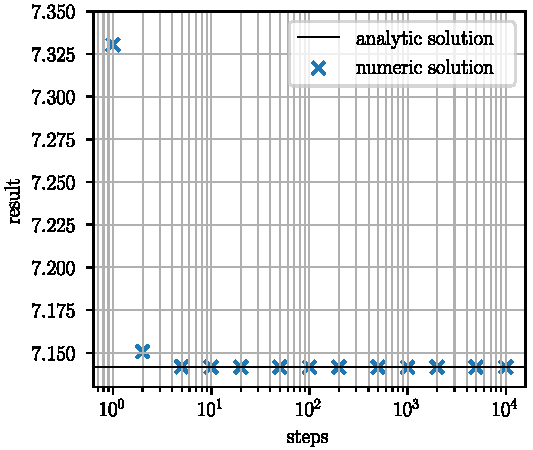
\includegraphics{../Task_01/simpson_results.pdf}}
    \caption{The result of the numerical integration of the integral in Equ.
    \ref{equ:test_integral}. The solid black line to the bottom represents the
    analytical solution of the integral which is \(\pi + 4 \approx 7.142\). Also
    apparent in this plot is, that the solution converges very fast. Using ten
    steps brings us already very close to the true solution.}
    \label{fig:Simpson_results}
\end{figure}

\section{Newton-Raphson solver}%
\label{sec:newton_raphson_solver}

One way to numercally solve an equation \(f(x) = 0\) with respect to \(x\) is
given by the following equation:
\begin{equation}
    \label{equ:newton_iterator}
    x_{i+1} = x_i - \frac{f(x_i)}{f'(x_i)}
\end{equation}
Here \(x_{i+1}\) is merely the next best approximation of the true result and
\(f'(x_i)\) is the first derivative of the function \(f(x_i)\). The
method, however, is in need of a initial guess of the solution. If there is only
one solution, this can be any number. But if there are more than one solution,
it is best to make a good guess that lies close to the desired solution. The
intrinsic nature of this method calls for a recursive approach, where the solver
function is called once by the user with the initial gues, and every following
invocation to further improve the approximation is done by the function itself,
with the new "initial" guess being the previous estimate. For this to work, we
need a break condition, or else the function would infinitely recurse. With
python this is not a big deal, as there are internal mechanisms preventing any
fatal errors to occure, unlike with other programing languages such as C++,
where this could lead to a segmentation fault. The main break condition used for
this problem is the difference \(|x_{i+1} - x_i|\) between two consecutive
estimators. Once the difference is less than a user defined tolerance, it is
assumed that the solution has converged.

The Newton method has been tested with two different equations:
\begin{eqnarray}
    f_1(x) =& x^3 - x + 1 &= 0 \label{equ:newton_test_1}\\
    f_2(x) =& \cos(x) - 2x &= 0 \label{equ:newton_test_2}
\end{eqnarray}
As initial guess, 0 was used for both equations. As can be seen in Fig.
\ref{fig:Newton_results}, the two solutions converge at different speed.
\begin{figure}[htbp]
    \resizebox{\hsize}{!}{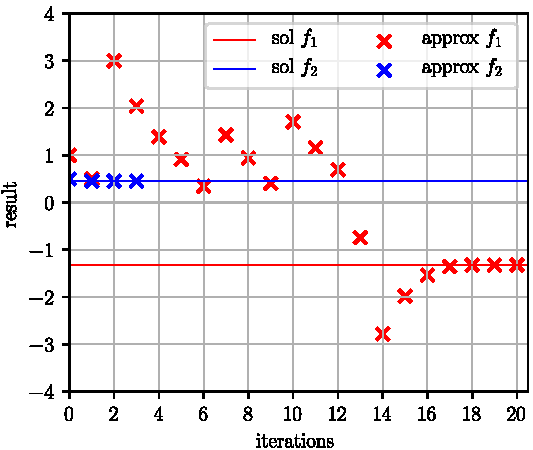
\includegraphics{../Task_02/newton_results.pdf}}
    \caption{The solutions of the two test equations Eqs.
    \ref{equ:newton_test_1} and \ref{equ:newton_test_2} converge after a
    different number of iterations. This is due to the fact that one solutions
    lies closer to the initial guess than the other. The solution for Equ.
    \ref{equ:newton_test_1} is \(-1.325\) and for Equ. \ref{equ:newton_test_2}
    it is \(0.450\).}
    \label{fig:Newton_results}
\end{figure}
To get to the solution of the first equation 21 iterations are needed. The
reason for this can be sought in the initial guess which is quite far from the
actual result. This is also a nice illustration of what could happen if there
was a second solution close to positive two. The algorithm may have found that
solution before it converged in on \(-1.325\).

\section{Bisection solver}%
\label{sec:bisection_solver}

Yet another method to solve an equation \(f(x) = 0\) with respect to \(x\). The
difference to the Newton solver discussed in Sec.
\ref{sec:newton_raphson_solver} is that it does not make use of the derivative
\(f'(x)\). However, an initial guess is not sufficient to this method. To
determine the solution of the equation, one must provide a range within the
solution can be found. A simple way to test if there is a solution in the
interval \([a, b]\) where one is suspected, is to compute \(f(a)\) and \(f(b)\).
If of the two results one is positive and the other is negative, they have
different signs, there is at least one solution between the boundaries of the
search interval. To narrow down the search interval, the midpoint \(c\) of the range
is computed and the function evaluated at that point.
\begin{equation}
    c = a + \frac{b - a}{2}
\end{equation}
Again the sign of \(f(c)\) is determined and compared to the signs at the
beginning and the end of the search interval. If the signs of \(f(a)\) and
\(f(c)\) are the same but differ from \(f(b)\) the solution lies in a new
interval \([c, b]\), if \(f(c)\) and \(f(b)\) have a different sign from
\(f(a)\) we expect the solution to be in the new interval \([a, c]\). Once
determined which new boundaries to use, a new midpoint is calculated and the
procedure is repeated so long until the result of \(f(c)\) approaches zero 
within a user defined tolerance.

As was the case with the Newton method, a recursive implemention is possible
where the function again calls itself with the new search interval as long as
the main break condition \(f(c) < \mathrm{tolerance}\) is not fullfilled.

\subsection{Parker wind}%
\label{ssub:parker_wind}

To test the bisection method, the Parker wind equation was used, see Equ.
\ref{equ:parker_wind}.
\begin{equation}
    \label{equ:parker_wind}
    v \exp \left(-\frac{v^2}{2c_s^2}\right) = c_s \left(\frac{r_c}{r}\right)^2
    \exp \left(- \frac{2r_c}{r} + \frac{3}{2}\right)
\end{equation}
However, to use the bisection method on this equation it had to be rarranged to
the following form.
\begin{equation}
    \label{equ:parker_alternate}
    c_s \left(\frac{r_c}{r}\right)^2 \exp \left(-\frac{2r_c}{r} + \frac{3}{2}\right)
    -v \exp \left(- \frac{v^2}{2c_s^2}\right) = 0
\end{equation}
n order to compute the windspeeds within \SI{1}{\AU} of the Sun,
\begin{figure}[htbp]
    \resizebox{\hsize}{!}{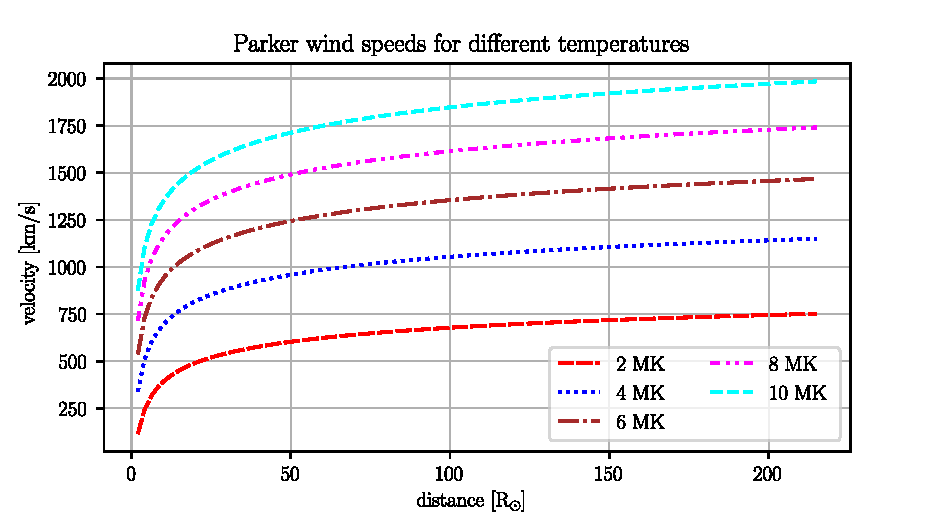
\includegraphics{../Task_03/parker_results.pdf}}
    \caption{An estimation of the windspeeds at different radii ranging from
    \SI{2}{\Rsol} to \SI{1}{\AU}. The progression was done for temperatures
    starting at \SI{2}{\mega\kelvin} with \SI{2}{\mega\kelvin} steps up to
    \SI{10}{\mega\kelvin}.}
    \label{fig:Parker_results}
\end{figure}

\end{document}
